\documentclass[12pt,letterpaper]{article}
\usepackage[latin1]{inputenc}
\usepackage{amsmath}
\usepackage{amsfonts}
\usepackage{amssymb}
\usepackage{graphicx}
\usepackage{hyperref}
\usepackage{parskip}
\usepackage{pdfpages}

\usepackage{fancyvrb} 

\usepackage{listings}

\usepackage{bm} 
\usepackage{xcolor} 

\xdefinecolor{gray}{rgb}{0.4,0.4,0.4} 
\xdefinecolor{blue}{RGB}{58,95,205}% R's royalblue3; #3A5FCD 

\lstset{% setup listings 
	language=R,% set programming language 
	basicstyle=\ttfamily\small,% basic font style 
	keywordstyle=\color{blue},% keyword style 
	commentstyle=\color{gray},% comment style 
	numbers=left,% display line numbers on the left side 
	numberstyle=\scriptsize,% use small line numbers 
	numbersep=10pt,% space between line numbers and code 
	tabsize=3,% sizes of tabs 
	showstringspaces=false,% do not replace spaces in strings by a certain character 
	captionpos=b,% positioning of the caption below 
	breaklines=true,% automatic line breaking 
	escapeinside={(*}{*)},% escaping to LaTeX 
	fancyvrb=true,% verbatim code is typset by listings 
	extendedchars=false,% prohibit extended chars (chars of codes 128--255) 
%	literate={"}{{\texttt{"}}}1{<-}{{$\bm\leftarrow$}}1{<<-}{{$\bm\twoheadleftarrow$}}1 
%	{~}{{$\bm\sim$}}1{<=}{{$\bm\le$}}1{>=}{{$\bm\ge$}}1{!=}{{$\bm\neq$}}1{^}{{$^{\bm\wedge}$}}1,% item to replace, text, length of chars 
	alsoletter={.<-},% becomes a letter 
	alsoother={$},% becomes other 
	otherkeywords={!=, ~, $, \&, \%/\%, \%*\%, \%\%, <-, <<-, /},% other keywords 
	deletekeywords={c}% remove keywords 
} 


\setcounter{secnumdepth}{0}  % don't number sections (stars not needed)




\author{Mark Novak}
\title{A quick and dirty intro to project structure, coding, and version control workflows}

\begin{document}
\maketitle


In what follows we'll talk about three things:
\begin{itemize}
\item How to structure your project(s)
\item Using \texttt{git} and \texttt{github.com} for version control
\item Best practices in coding
\end{itemize}

\pagebreak

\tableofcontents

\pagebreak

\section{Project structure} \label{projectsetup}
The general recommendations of this section in regards to establishing a consistent structure for your project(s) should apply whether or not you plan to use version control software to manage your project(s) or not.  For example, the recommendations apply equally if you plan to use \texttt{Dropbox} or the equivalent (which you should \emph{most definitely} be using if you're not going to use version control software).

Like many grad students, I finished my thesis with
\begin{itemize} 
	\item one master folder called \texttt{Data} containing a bunch of sub-folders within it containing all the various data sets (mostly Excel and CSV files) and databases (mostly MS Access) that I'd collected or collated over the years;
	\item one master folder called \texttt{Rcodes} containing a bunch of sub-folders within it (each with a different project or analysis of my data);
	\item one master folder called \texttt{Mathematica} that similarly contained a bunch of sub-folders;
	\item one master folder called \texttt{Manuscripts} that contained all the papers and chapters I'd attempted, completed or published;
\end{itemize}
and a bunch more similar folders all variously named within my overall \texttt{Research} folder.  You might currently have something similar for just your Thesis.

Turns out that's a poor way to organize your work for a variety of reasons, including reproducability (by yourself down the road or someone else if you managed to pull all the necessary parts together for that person); the ease and efficiency with which you might expand, modify or branch off of prior work; and the ease of performing data and code backups.

I now organize my work using a \emph{project mindset}.  I don't do this for each and every project idea or analysis I try out, but I do use it for ``definitely doing this'' (i.e.  planned out paper (thesis chapter)) and collaborative projects.  By \emph{project mindset}, I mean that everything associated with a given project is contained in one folder.   I still use a combination of \texttt{Dropbox} and \texttt{git} to organize my projects (and you should \emph{never} put a \texttt{git} folder within your \texttt{Dropbox} folder, or vice versa), but within each of either \texttt{Dropbox} or \texttt{git} I have all my project folders organized within a master \texttt{Projects} folder.   

That said, defining ``a project'' can get difficult (esp. within your thesis work), so a fair bit of forethought can be needed.  It's not trivial.

Ben says: I also use \emph{project mindset} to organize my folders.  Something I like about project mindset is that it encourages what you might call deliverables-based thinking. By identifying and naming the ``definitely doing this'' projects, I am encouraged to consider my priorities, both within and among projects. 

For each project I am forced to think clearly about what it is about by needing to name the folder. Asking ``what should this project folder (or Git repo) be called?'' (and insisiting on an \emph{informative name}, eg not ``MarkBencoursething'') is pretty close to asking ``what is this project about?'' So project organization supports clear scientific thinking. 

I find project mindset also promotes better time management. For instance, all my project folders are contained within three superfolders: Active, Complete and Archive. The folders within Complete are named with dates and brief titles of publication. The Active folder contains stuff I am working on right now, that has not ``shipped'' yet. Archive is for stuff that is on the back burner. 

In this setup, the project folders within the Active folder, each with a name that reminds me of the objective for that project, becomes a kind of high-level to-do list. The goal is to be able to one day drag those folders from Active to Complete. Crucially, if the Active folder gets too full, I know I will not be able to do that because my attention has become too divided. So then I ask myself which are the most important few projects to me, and drag the rest to the Archive folder. It's not that I can't do them later. It is just recognizing that a) they are not done yet, and b) they are not the first, second or even third priority. If a) and b) are true, into the Archive folder they go!

OK, back to Mark, and the structure of an individual project folder.

\subsection{Your Project folder / Respository} \label{projectfolder}
Within each project folder I  usually have the following sub-folders:

\begin{tabular}{ll}
 \texttt{data} & The original (and cleaned) data required for the project\\
 \texttt{code} & All the scripts needed to perform the analyses \\
 \texttt{output} & The results of the analyses \\
 \texttt{figures} & The final figures (and tables) that go into the manuscript\\
 \texttt{manuscript} & Manuscript(s) derived from the project\\
 \texttt{pdfs} & (\emph{as appropriate}) Collection of relevant papers, manuals, etc.\\
 \texttt{biblio} & (\emph{as appropriate}) Bibliographic files\\
\end{tabular}

The last two (\texttt{pdfs} and \texttt{biblio}) sometimes get put in sub-folders within the \texttt{manuscript} folder.  The  \texttt{manuscript} folder often contains sub-folders, one for each journal I've submitted to.  The \texttt{figures} folder sometimes gets put within each of the  \texttt{manuscript} sub-folders, depending on how much I decide to change what the final figures are for different journals.  The contents of \texttt{figures} differs from the rough-and-dirty figures I save into the \texttt{output} folder.  Sometimes \texttt{tables} get their own folder (if there are a lot of them). 

Ben says: My sub-folder structure is similar to what is listed below, with variations depending on the project and preferences. For example, my reference manager of choice keeps all my pdfs in one place, so instead of having a pdfs folder in each project folder, I have 'folders' for each project within my reference manager. Either way, the same goal is achieved: a logical hierarchical structure that makes it easy to find and keep the various pieces of a project. Back to you Mark.

Most of the time when using \texttt{git} you'll have one \emph{repository} associated with each one of your \emph{projects}.  A \emph{repository} as thus synonymous with a \emph{project folder}.  When using \texttt{git} you'll also have a few other files within the repository: a \texttt{README.md} file and a \texttt{.gitignore} file.  If you're using \texttt{R-Studio} in combination with \texttt{git} (as we will below), then you'll also have an \texttt{.Rproj} file in the repository.

\pagebreak

\section{Working with \texttt{git}}

\subsection{What is version control?}
Version control software allows you to save and provide meta-information on any and all changes you make to a set of files and directories.  It allows you to more easily document changes and the evolution of your files, find and correct bugs that have crept into your code, and revert back to old file versions when needed.  By using version control you'll now what, when and (hopefully) why changes were made.  If you're using the software collaboratively, you'll also know by whom changes were made.  Backing-up is virtually implicit (though not totally so), especially when you also use a networked (off-site) server as a host for your repository.

We'll be using \texttt{git} as our version control software.  There are others out there (e.g., \texttt{Subversion}).  We'll also be using \texttt{Github} as our host.  There are others out there (e.g., \texttt{Bitbucket}).

\subsection{git}
\texttt{git} was developed by Linus Torvalds (the ``Linu'' in Linux).  Most of its features are accessed by command-line and are intended for large-scale collaborative programming and software development purposes.  Of course, we'll be using \texttt{git} for much smaller, specific projects, thus we won't bother with many of these feature.  We'll also interact with \texttt{git} using GUIs (e.g., \texttt{R-Studio}) rather than command-line.  

\textbf{Required reading} to get an overview of how \texttt{git} works:\\
\url{https://git-scm.com/book/en/v2/Getting-Started-What-is-Git%3F}.

\subsection{Github}
\texttt{Git} enables you to store a complete copy of the project on your local machine, including its history and all versions.  That means that no centralized server is necessary.  However, if you want to collaborate with others, have multiple computers with which you'd like to work, or want to create true back-ups of your project, then you'll also want to use a server on which to host your repository.  Fortunately, there are a number of free providers. 

For \texttt{git}, the primary options are \texttt{Github} and \texttt{Bitbucket}.  The former is more developed (more bells and whistles), is currently more widely used, and is perhaps a little easier to work with.  The two don't differ all that much except in one regard:  the number of free versus public repositories.  While \texttt{Github} has a limit on the number of private repositories, \texttt{Bitbucket} has a limit on the number of collaborative projects (having more than 5 collaborators).  (There may still be perks regarding the number of repositories when you sign up using an academic email address.)

\textbf{To do:} Create an account on \texttt{github}.  (I suggest creating accounts with both hosts.  I use them for different projects, as needed.)


\subsection{Installing and configuring Git}
To install and configure \texttt{git} on a PC, go see \\
\url{https://git-scm.com/book/en/v2/Getting-Started-Installing-Git}

To install \texttt{git} on a Mac:

\url{http://code.google.com/p/git-osx-installer}\\
or\\
\url{http://git-scm.com/downloads}


After you install \texttt{git} there's a little (minimum of) command-line configuration to perform.  On a Mac, open a \texttt{Terminal} window and type in the following:

     \texttt{\$ git config --global user.name "Mark Novak"}\\
     \texttt{\$ git config --global user.email "Mark.Novak@oregonstate.edu"}
       
Some of you might want to set up an editor to be used in git, for example:

	\texttt{\$ git config --global core.editor emacs}

You can check to ensure that these commands when through and see what other things you might want to configure using

	\texttt{\$ git config --list}


For more, see\\
\url{https://git-scm.com/book/en/v2/Getting-Started-First-Time-Git-Setup}


\subsection{Repository setup}
There are command-line methods for doing everything we're going to do below.  Indeed, command-line is the default way that most people interact with \texttt{git}. (See last page for a cheat sheet.)  Instead, we're going to make use of the tools made available through \texttt{Github}, starting with the very first step of initiating a repository and getting some minimal information associated with it.  That is, rather than creating and setting up a repository on our computer by command-line and then connecting it to \texttt{Github}, we'll create and set it up on \texttt{Github} and clone it to our local  master folder of projects.

Simply log in to your \texttt{Github} account, click on ``New Repository'', and follow the instructions.  These should include options for private versus public (pick the latter for this class), initializing with a \texttt{README} file (which you \emph{should} do), and adding a \texttt{.gitignore} file (which you \emph{should} also do).

The \texttt{README} file is the first file that anyone will look at when they inspect your repository (assuming it's public).  It should give an overview of what the project is about and what the various parts of the project structure are.  You can edit it at any time, but for now put some minimally useful information in it.   The \texttt{.gitignore} file contains a list of all the files that you want \texttt{git} to ignore (not monitor for changes).  Selecting \texttt{R} from the dropdown list will auto-fill a bunch of it for you.  You typically won't do much with this list, though it is useful sometimes.  (For example, you may wish to have \texttt{git} ignore (not manage) the \texttt{.Rproj} file that \texttt{R-Studio} creates.)

You should now see a new webpage -- your Repo page -- that shows you what's in your repository.  For now it contains only the  \texttt{.gitignore} and \texttt{README.md} files, the latter of which has its contents displayed.  As I said earlier, there's a lot of bells-and-whistles at your fingertips here (the most useful of which for collaborative projects is the \texttt{Issues} feature).  You \emph{could} start dragging-in directories and files to add them to your repository, but we're \emph{not} going to do that.  Instead, we're going to \texttt{clone} this repository to our local machine, then add our various project sub-folders to it (from \nameref{projectfolder}) and go from there.

To clone the repository, click the green \texttt{Clone or download} button and copy the provided URL.

Now there's a couple ways to clone your repository to your local machine.  The preferred method depends on how you're most likely going to interface with \texttt{git}.  You could:
\begin{enumerate}
	\item use command-line to clone.  Open \texttt{Terminal}, \texttt{cd} into your \texttt{Projects} master folder, then type \texttt{git clone} followed by the URL;
	\item use a visual \texttt{git} GUI client to clone the repo;
	or, if you're going to be primarily using \texttt{R} via \texttt{R-Studio} anway,
	\item set up a ``project'' within \texttt{R-Studio} first and provide it with the URL during setup.  It'll then clone the repo for you.
\end{enumerate} 

\subsection{R-Studio and Git GUIs}
I use \texttt{git} for both \texttt{R} and non-\texttt{R} (e.g.,  \texttt{Mathematica})-based projects.  Only  \texttt{R-Studio} has integrated  \texttt{git} functionality, so I use a visual  \texttt{git} GUI client (e.g., \texttt{Sourcetree}) for some projects because I can't be bothered to memorize the  \texttt{git} command-line commands.  Since most of you are probably using \texttt{R}, it's probably worthwhile to use \texttt{R-Studio}'s  \texttt{git} integration feature (which is the only reason I use  \texttt{R-Studio} to begin with).

You'll first need to tell  \texttt{R-Studio} that you have \texttt{git} installed, so go to its Preferences, select \texttt{Git/SVN} and fill in the details: either click on the Help link or go to 
\url{http://r-pkgs.had.co.nz/git.html} to see what to do.

Now create your ``project'' within  \texttt{R-Studio} by selecting ``New Project''.  Select \texttt{Version Control: Checkout a project from...repository}, select \texttt{git}, and fill in the details including the URL you got from \texttt{Github}.  The directory in which you place your repository should be your master folder.   \texttt{R-Studio} will ``restart'' and then you'll be in your project (as evidenced by its name appearing in the top-right of the interface).  Clicking on the \texttt{Files} tab will show you what's in the repository (which should at present be: \texttt{README.md}, \texttt{.gitignore} and the newly created \texttt{.Rproj} file).

You may now create (or move in) all your project sub-folders  (see \nameref{projectfolder}).


\subsection{Git work flow}
First, \textbf{required reading:}\\
\url{https://git-scm.com/book/en/v2/Getting-Started-What-is-Git%3F}

Basically, files (or directories) exist in one of four states of a life-cycle: untracked, staged, unmodified, or modified (see Fig. \ref{fig:lifecycle}).  The standard workflow is thus:
\begin{enumerate}
	\item Add or modify some files.
	\item Stage the new or modified files.
	\item Commit the changes (moving them from the Staging Area to the ``memory'' of the repository).
	\item Repeat.
\end{enumerate}

\begin{figure}
	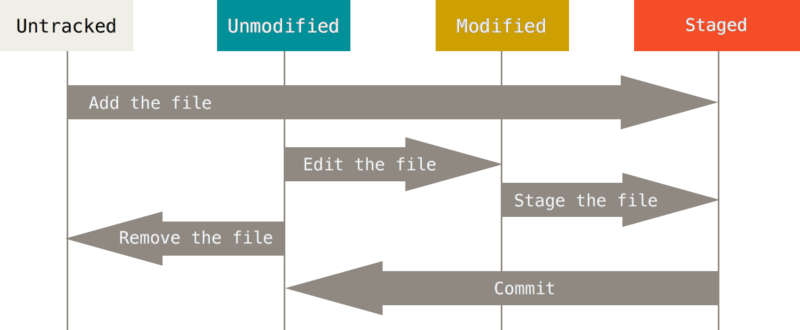
\includegraphics[width=\linewidth]{figs/lifecycle.png}
	\caption{The \texttt{git} life-cycle.}
	\label{fig:lifecycle}
\end{figure}

The motto of \texttt{git} is ``\emph{commit early, commit often}''.  Every time you add or remove something from your project (i.e. a file or a chunk of code), you want to commit those changes.   Ideally, each commit should correspond to a ``logical unit'', one that you are able to describe in a few words (e.g., ``function to perform resampling added to analysis script''). Choosing when to commit is quite important, especially when you're debugging code:  For example, if you've discovered your code has two bugs then you should commit each one of the fixes seperately, not together.  That way you can undo either fix independently if, for example, you messed up in one of your fixes or your fix created a different bug somewhere else in your code.

Within \texttt{R-Studio} (and assuming you have your \texttt{R-Studio} project opened), looking at the \texttt{git} tab will show you a list of all the files (and directories) that have been changed, removed or added to the project since the last time you committed.  Clicking on the check-boxes associated with each file will add them to the staging area.  Clicking on \texttt{Diff} or \texttt{Commit} will open up a new interface (the staging area).  In the top-left corner you'll see a list of the staged files.  Selecting one of the files will bring its contents up in the window below which highlights the text that has been added (in green) and removed (in red).  Select all the files you want to commit, then add a commit message to the top-right window, and commit.  

You've now updated your local respository.  Clicking on \texttt{History} (top-left) will show you all your past commits.  Remember, ``\emph{commit early, commit often}''.


\begin{figure}
	\centering
	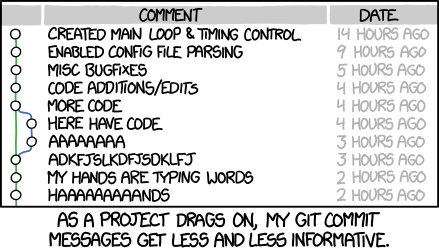
\includegraphics[width=0.5\linewidth]{figs/xkcd_git_commit.png}
	\caption{Don't let this happen!  (source: \url{http://xkcd.com/1296/})}
	\label{fig:commit_messages}
\end{figure}

The final thing to do (often, for back-up reasons, but not necessarily following each commit) is to \texttt{Push} your commit to \texttt{Github}.  \texttt{Pull} obviously does the opposite: bringing commits that have been saved to \texttt{Github} (by others, or by you on a different machine) to your local machine.

\emph{ \textbf{Note:}  To avoid conflicts, the safe thing to do is to always pull before you start making edits, commit and push.  There are of course ways of dealing with conflicts and merging files (that will arise if two people are working on the same file, for example), but for our mostly single-user purposes it's easier to just avoid them.}


\subsection{Git resources}
There's a whole lot more functionality to \texttt{git}, some of which is important and very useful (such as resolving conflicts, branching and merging, and reverting back to old versions), but we're not going to get into that unless we have extra time.  For more information, check out the following resources:

\url{https://www.codecademy.com/learn/learn-git}\\
\url{https://www.atlassian.com/git/tutorials}\\
\url{http://rogerdudler.github.io/git-guide/}\\
\url{https://git-scm.com/book/en/v2}



\pagebreak


\section{Coding}
The reality is that for any non-trivial task, most of your time will be spent de-bugging your code, not writing it.  There are two over-arching principles that will, when practiced, greatly increase your efficiency:  writing \emph{modular} code and writing \emph{clean} code.  In class we'll discuss modularity first (it relates to the \emph{project mindset} referred to in the context of \texttt{git}) and will then talk about code-writing best practices (styles guides).

\subsection{Principle of Modularity}
If your experience learning to code as been anything like mine then, either when you first started coding or when you wrote homework assignments for Stats class, the code you created for a given project probably consisted of one long giant file.  If you learned to use \texttt{Markdown} or \texttt{Sweave}, that code probably had some number of sections within it, just like you might write a paper or thesis chapter (Intro, Methods, Results).  

That'll work fine for small (tiny) projects or homework reports, but probably not for anything the size of a paper or thesis chapter that contains some combination or subset of data, analyses (whether statistical or non-statistical modeling), and data- or results visualization.

Thus, as alluded to in \nameref{projectfolder}, you should give your project a useful structure:

Your \texttt{data} folder should contain all the data you need for the project.  Most of the time, this will include both the \emph{original} unedited raw data files (regardless of their format) as well as \emph{derived} data files (that you have used code to produce).  No files should be duplicates or derived copies of each other (see Fig. \ref{fig:datafilenames}); remember: versions will be tracked by \texttt{git}. 

Your \texttt{code} folder contains your various script files.  For anything but the smallest projects there should be multiple files that contain scripts for performing different tasks.  For example, you might have: 

\begin{tabular}{p{0.2\linewidth}p{0.8\linewidth}}
	\texttt{data\_prep.R} & Script that pulls in the original data, pre-processes them (rearranges, correct errors, standardizes names, splits up or merges different data sets), and spits them back out in a ``clean'' format needed by your subsequent analyses \\
	\texttt{my\_functions.R} & Script containing the functions you have self-defined to perform your analyses \\
	\texttt{analysis.R} & Script that sucsk in your ``clean'' data, performs your analyses (using built-in, self-defined and package functions), makes some quick-and-dirty figures along the way, and exports the results to \texttt{output} \\
	\texttt{final\_figs.R} & Script that sucks in the results of the analyses to produce the final figures (or tables) for your manuscript\\

\end{tabular}

In general, you don't want any file to become unwieldy.  Thus you will likely have multiple scripts within each of the above categories (e.g., one for each of several different data set types, one for each of several different analyses or analysis steps, or one for each of several different self-defined functions) -- each appropriately named (see \nameref{codestyleguide}).  If you end up with a whole lot of scripts to perform an analysis from start to finish, then you may want one additional \texttt{RunMe.R} script that sources each of the other scripts in the appropriate order.


The key utilities of separating out everything as specified above are (1) \emph{readability} and (2) \emph{unit-testing}.    Readability means that it's easy for anyone (including you in 1 years time) to figure out where things are being pulled from and where they're going, and no individual script is overwhelming to look through.  The idea behind unit-testing is to write independent tests for the smallest units of your code.  For example, whenever you write a function, you also write an associated small piece of code that tests it (before the function is used in your primary analysis). That way, whenever you modify your code or function(s), it's easy to ensure that everything is still returning the correct output.



\begin{figure}
	\centering
	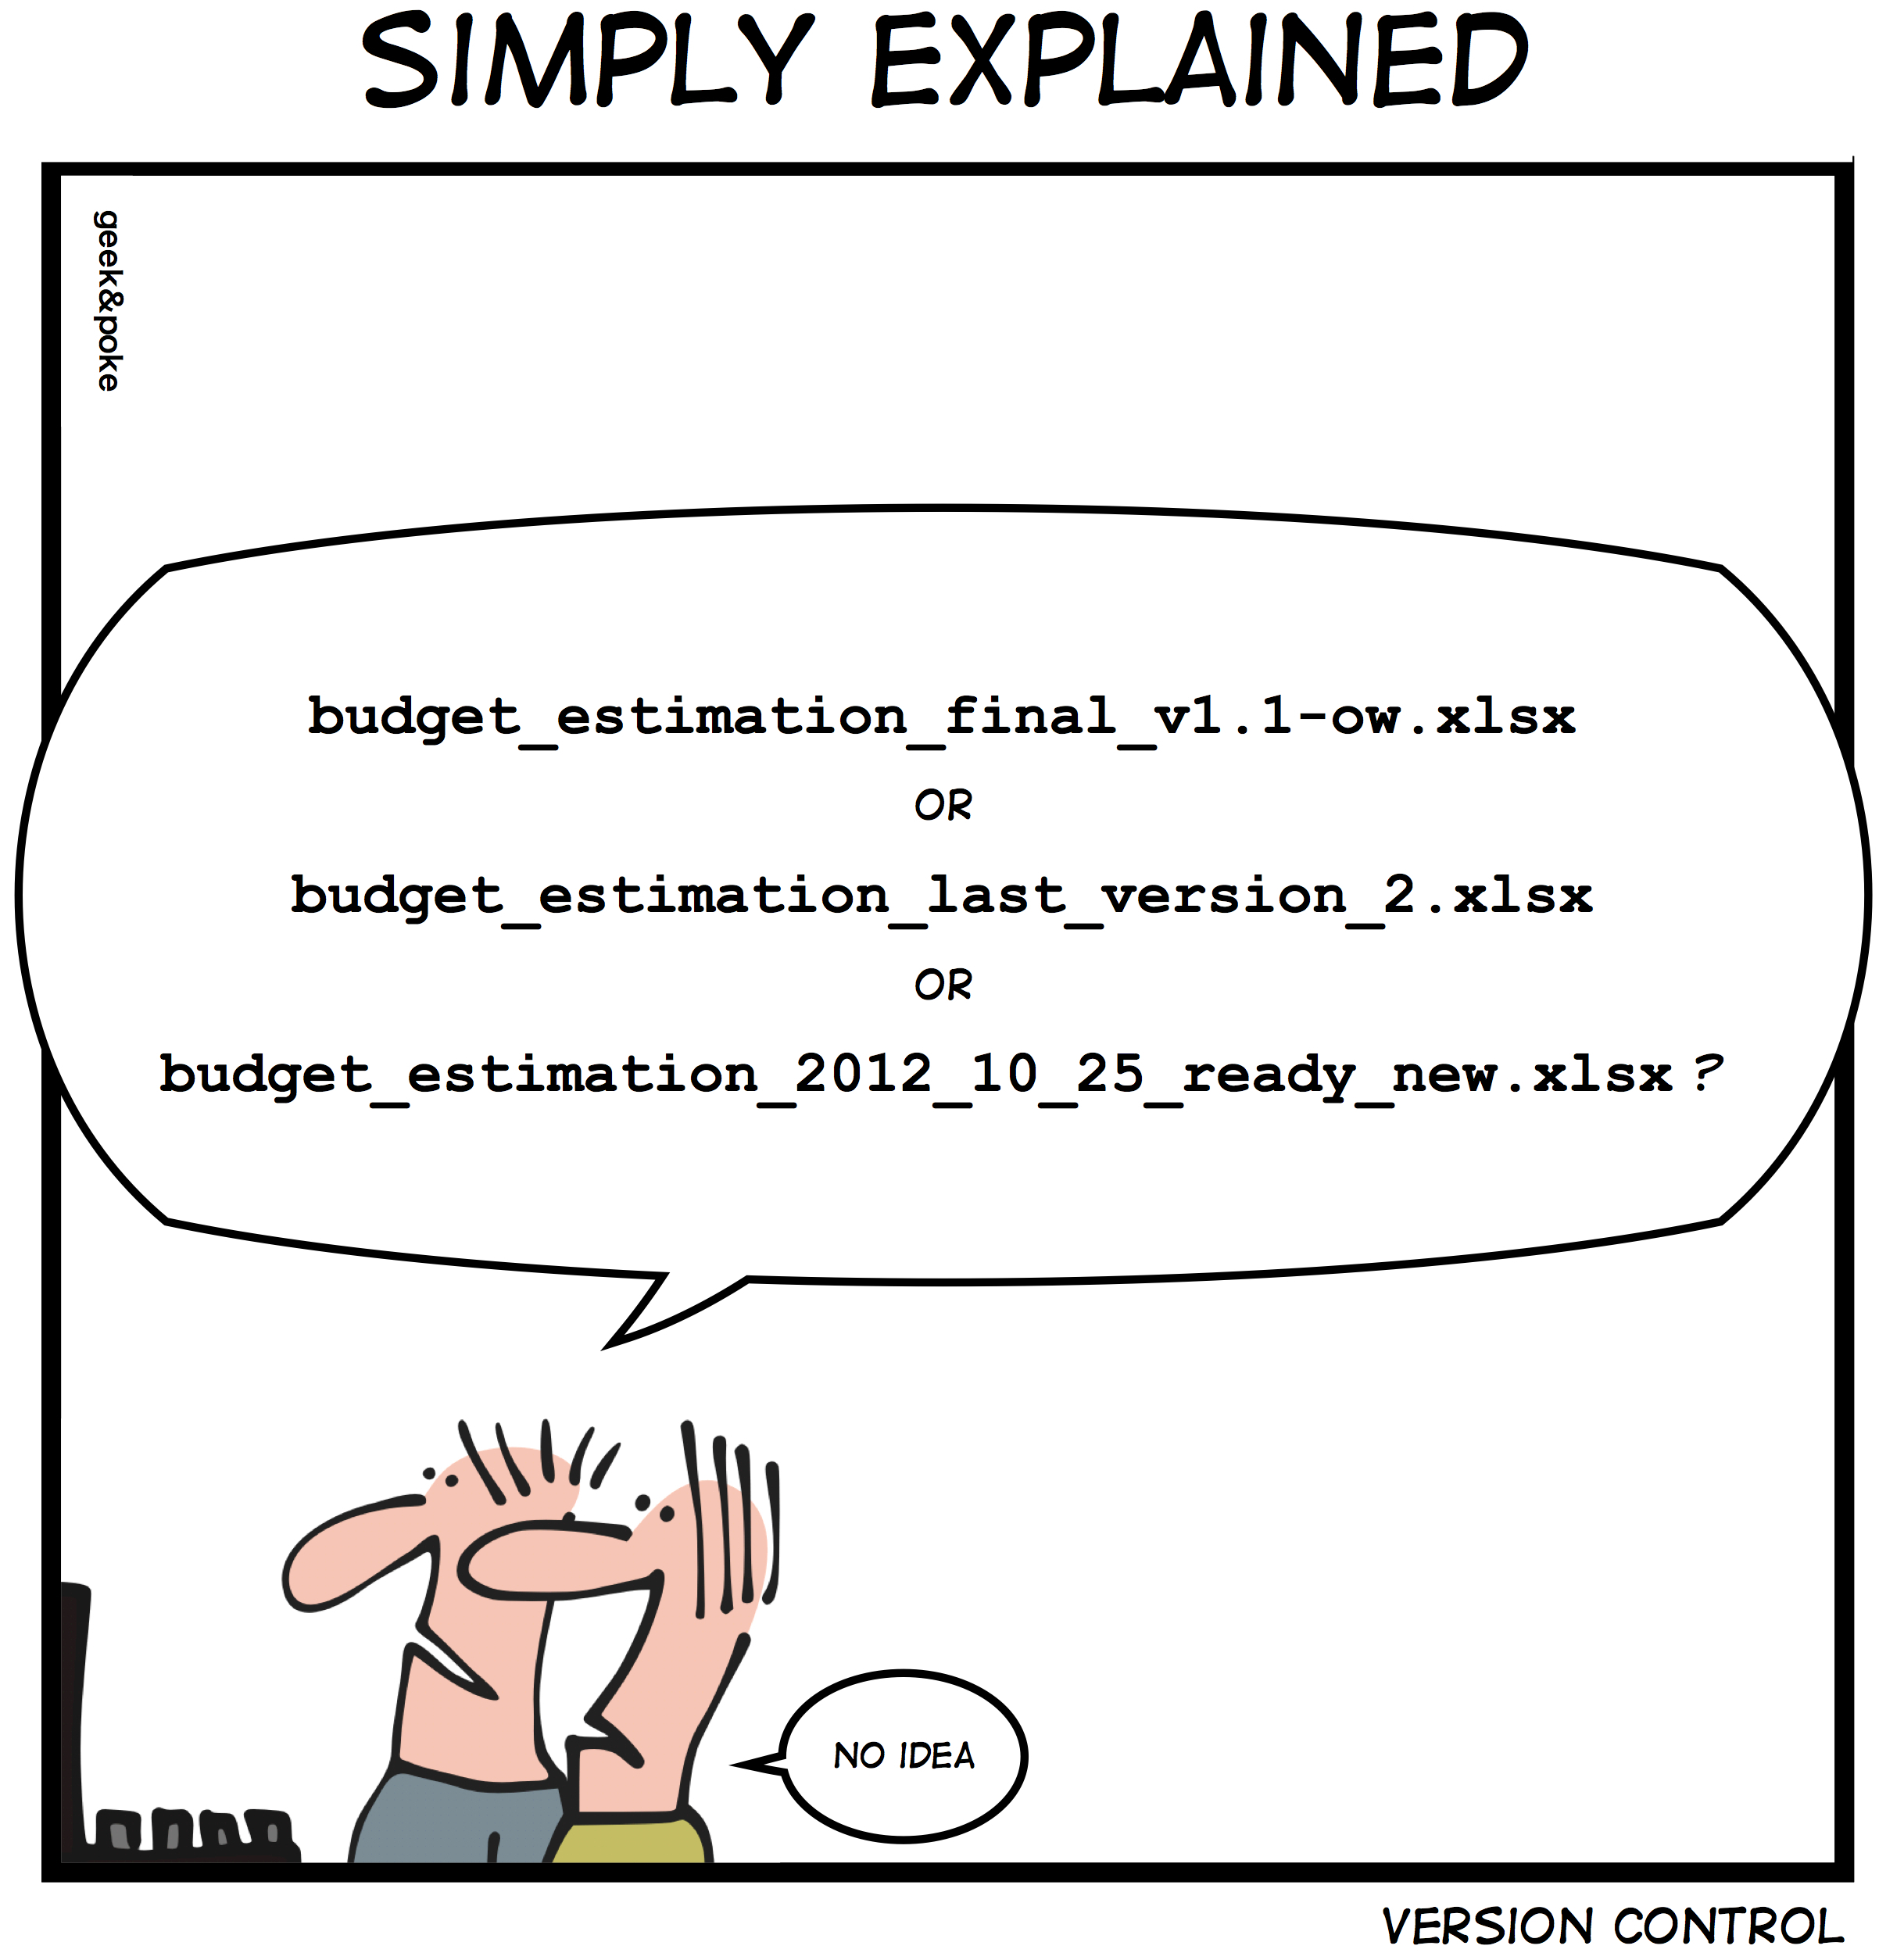
\includegraphics[width=0.5\linewidth]{figs/datafilenames.jpg}
	\caption{Never again should your data files look like this!}
	\label{fig:datafilenames}
\end{figure}

\subsubsection{Working directory and directory access}
In order to employ the principle of modularity you need to know how to navigate between your various folders and scripts.  Within a project, for example, you have a choice between using the repository folder as your working directory or setting your working directory to be the directory in which you have saved your scripts (e.g., your RunMe script). Your scripts will therefore need to access data and source scripts that are located in other folders.  You want to set these locations as generically as possible (so that you can move your entire project to a different location without destroying the workflow, for example).  You never want to set the working directory more than once, or hard-write the locations of your data or other scripts within a given script.  

You can do this by specifying locations relationally using `\texttt{/.../file.R}', for example. Each repetition of `\texttt{/.../}' will move you up one level in the folder structure.   For example, assuming your working directory is the \texttt{code} directory, rather than specifying the location of your data as

\texttt{read.csv(file=`C://MyDocuments/Git/MyProject/data/data.csv')}

you should instead use

\texttt{read.csv(file=`.../data/data.csv')}.

The latter takes you up one level (out of \texttt{code} into your general \texttt{repository} folder) then into the \texttt{data} folder and to your data file.  To pull in scripts, use 

\texttt{source(file=`my\_functions.R')}

(assuming your working directory is the \texttt{code} directory).

\textbf{Note:} Macs (Unix) and Windows (Dos) use forwardslashes and backslashes differently.  Macs use `\texttt{/.../.../file.R}' (forwardslashes) while Windows use `\texttt{\textbackslash...\textbackslash...\textbackslash file.R}' (backslashes).


\subsection{Code style guides} \label{codestyleguide}
There are a lot of summarized sets of recommended best-practices for coding in general and for \texttt{R} as well.  These includes aspects relating to object naming conventions (for filenames, function names, and variable names), syntax and grammar (spacing, indentation, etc.), and code structure.  I won't repeat everything here, but we will go over and discuss the big ones in class.  For our course, the \textbf{required reading} is:

\url{https://google.github.io/styleguide/Rguide.xml}

Other guides that are well worth reading for some additional suggestions and explanations are:

\url{https://www.r-bloggers.com/r-code-best-practices/}

and 

\url{http://adv-r.had.co.nz/Style.html}


\subsection{Within-script organization}
In additional the best practices in the naming of objects and the syntax of your code, there's also an important aspect of within-code organization. Your code should consist of the following sections, each visually separated from the others:

\begin{enumerate}

	\item Start each file with a preface that describes what it contains and how it fits into the project. You might also want to include who wrote it and when.
	
	\item Load all required packages
	
	\item Source required scripts (e.g., \texttt{my\_functions.R})
	
	\item Load (or source) required data (or \texttt{data\_prep.R} scripts)
	
	\item Section(s) for major parts of your analyses
	
	\item Export results section(s)

\end{enumerate}
The last two may consist of just two sections or may have export parts immediately following an analysis.  Wherever possible and appropriate, clear your workspace (\texttt{rm(list=ls())}).  For example, you'd most definitely do this at the top of your \texttt{RunMe.R} script and perhaps to at the top of your \texttt{analysis.R} script (since your ``cleaned'' data was saved and can be reloaded, leaving all the temporary variables unnecessary), but you wouldn't put \texttt{rm(list=ls())} at the head of your \texttt{my\_functions.R} script.

Thus a script file might look as follows:

\noindent\rule{12cm}{0.4pt}
\begin{lstlisting}[language=R]
########################################################
# simulateLV.R
# Simulates the dynamics of a predator and prey population according to the Lotka-Volterra model.  
# The data produced will subsequently be used to test the performance of several population dynamic model-fitting routines.
########################################################
rm(list=ls()) # clear workspace

##############################
# Load librairies
##############################
library(deSolve)

############################## 
# Source files
##############################
# None needed

##############################
# Define model
##############################
LVmod <- function(Time, State, Pars) {
	with(as.list(c(State, Pars)), {
		Ingestion    <- rIng  * Prey * Predator
		GrowthPrey   <- rGrow * Prey * (1 - Prey/K)
		MortPredator <- rMort * Predator
		
		dPrey        <- GrowthPrey - Ingestion
		dPredator    <- Ingestion * assEff - MortPredator
		
		return(list(c(dPrey, dPredator)))
		})
	}

##############################
# Define parameters
##############################
pars <- c( rIng   = 0.2,    # /day, rate of ingestion
	      rGrow  = 1.0,    # /day, prey growth rate
	      rMort  = 0.2 ,   # /day, predator mortality
	      assEff = 0.5,    # assimilation efficiency
	      K      = 10)     # mmol/m3, carrying capacity

##############################
# Simulate model
##############################
yini  <- c(Prey = 1, Predator = 2)
times <- seq(0, 200, by = 1)
out   <- ode(yini, times, LVmod, pars)
summary(out)

##############################
# Plot and export data
##############################
plot(out)
write.csv(out, file=`.../output/LV_out.csv')

##########################################################
\end{lstlisting}
\noindent\rule{12cm}{0.4pt}

When defining a function, you should provide additional information that describes what the function does (in general terms), what inputs it takes, and what output it returns.  After the function is defined it's worth adding a test case (commented out).  [Note: some would separate out test cases, leaving only the function definition in its own script.]  For example:

\noindent\rule{12cm}{0.4pt}
\begin{lstlisting}[language=R]
########################################################
# Function to add stochastic noise to a time-series of population sizes.
########################################################
# Input:
#	x -- a time series of population sizes (vector)
#	error_model -- gaussian (currently implemented model, default)
# 	sd -- the standard deviation of gaussian errors (default=0)
# Returns:
#	Vector of length equal to the input vector of time series

add_error <- function(x, error_model=`gaussian', sd=0){
	error_model <- match.arg(error_model)
	if(error_model==`gaussian'){
		out <- x + rnorm(length(x), sd)
	}else{
		out <- x
		warning(``Original time series returned'')
	}
	return(out)
}

# Test:
# source(`simulateLV.R')
# new <- add.error(out, sd=1)
# par(mfrow=c(1,2))
#	plot(out)
#	plot(new)
\end{lstlisting}
\noindent\rule{12cm}{0.4pt}


\subsection{When writing code, though shalt not...}

\begin{itemize}
\item Copy-paste-edit (i.e. reuse and modify) the same code to repeatedly apply it to different subsets of data, etc..  Instead, you will convert your code to function(s) that can be applied to these data subsets
\item Use \texttt{attach()} and \texttt{detach()} on your data.  Instead, be explicit in naming and accessing data.frame columns.
\item Repeatedly reset your working directory.  Instead, use relational sourcing.
\item Save your \textsf{R} workspace for later reuse.  Instead, use \texttt{rm(list=ls())} wherever possible and appropriate.
\item create large tables by hand. If you find yourself having to export large tables a lot, learn \LaTeX and export them instead
\end{itemize}


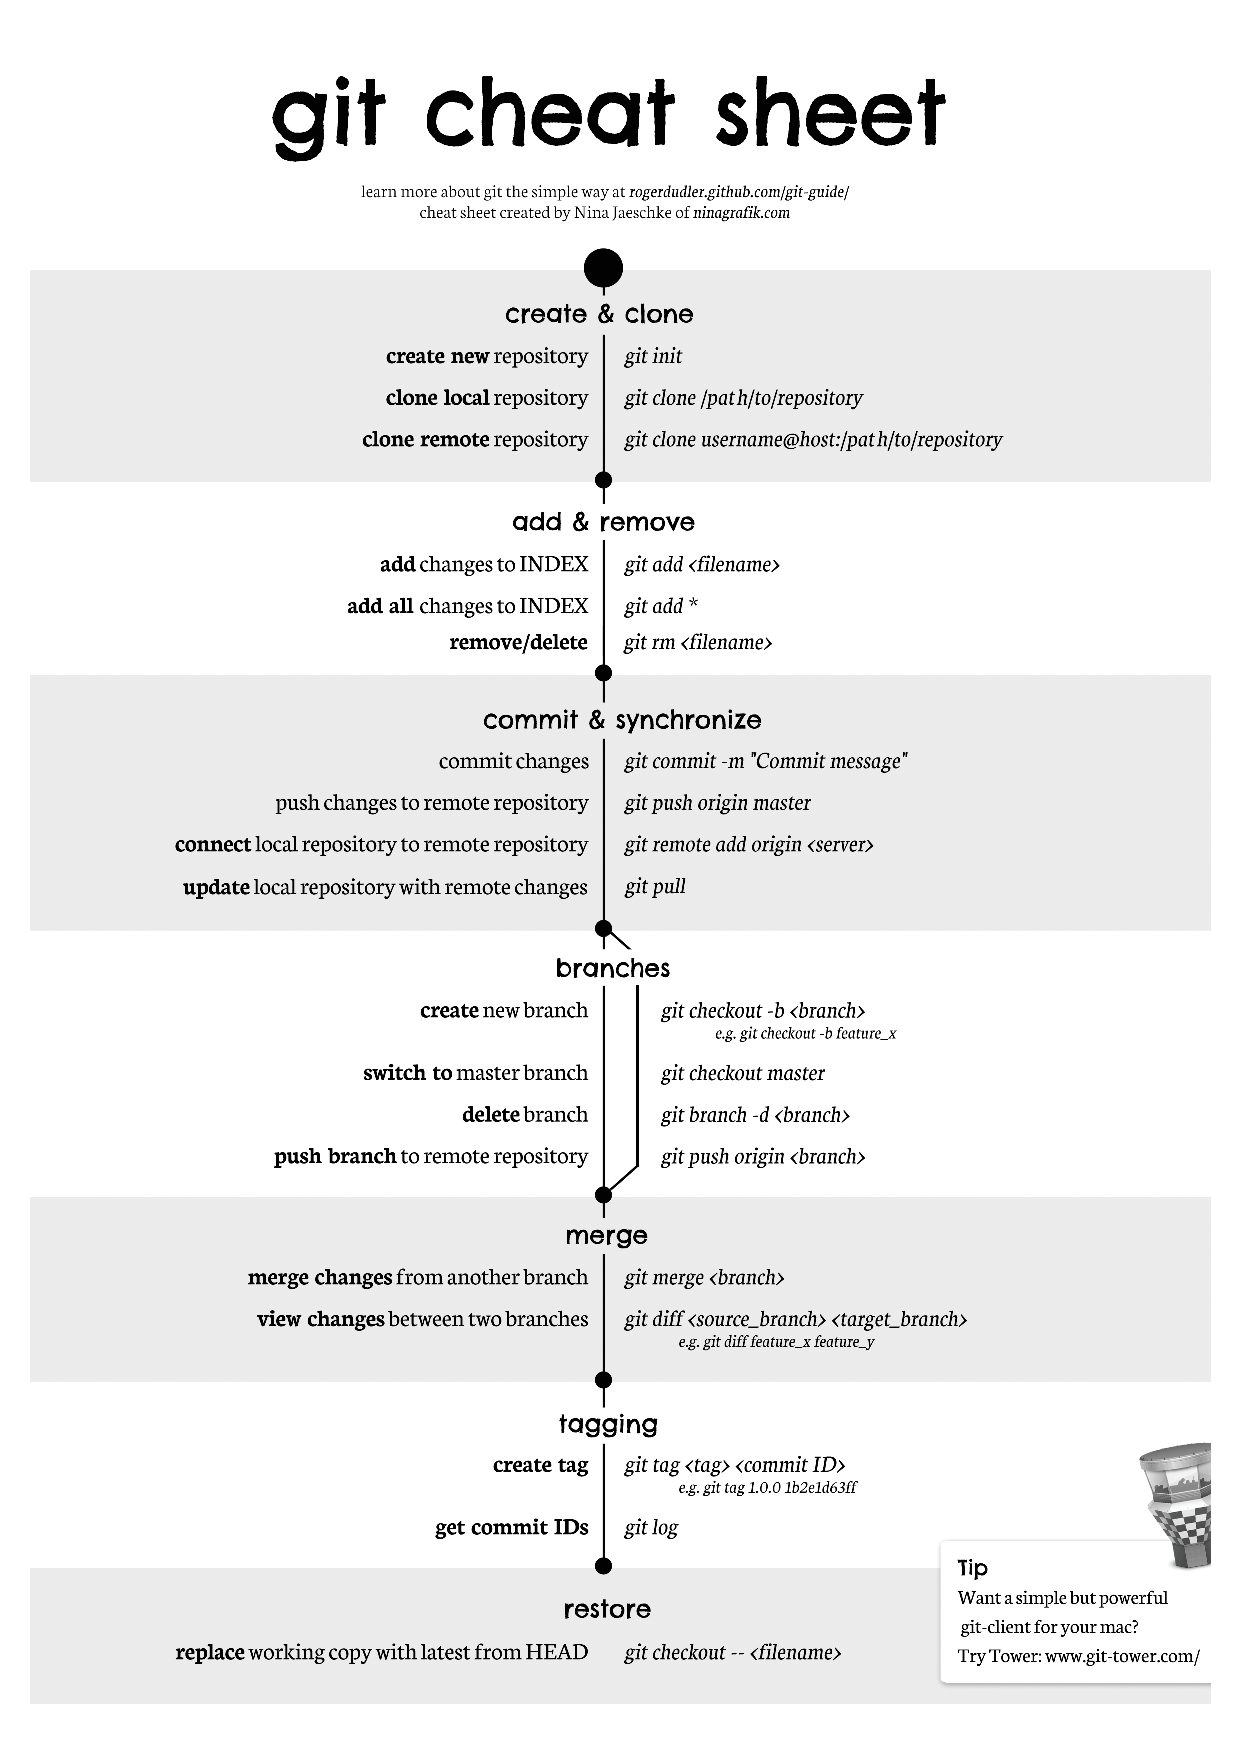
\includepdf{figs/git_cheat_sheet.pdf}

\end{document}